\chapter{Análisis del Montaje Experimental}
\label{sec:analisis_montaje}

El montaje experimental presenta simetrías notables que determinan los
posibles efectos a observar.

Independientemente de la dirección relativa de los campos magnéticos
generados por cada par de bobinas coaxiales, el sistema exhibe una
simetría de reflexión respecto a los planos $xz$, $yz$ y $xy$.
Esto se debe a la simetría axial intrínseca de las bobinas y a su disposición
simétrica respecto al origen.

Además, si ambos pares de bobinas operan a la misma frecuencia, se
obtiene una simetría rotacional de $\pi/2$ en el plano $yz$.
En el caso general de frecuencias distintas, esta se reduce a una simetría de
rotación de $\pi$.
Estas simetrías son fundamentales para la construcción de los modelos teóricos
y la simplificación de los cálculos.
Por tanto, se espera que los patrones observados en la pantalla reflejen estas
mismas simetrías.

\section{Modelos Clásicos con Álgebra Geométrica}
\label{sec:modelo_clasico}

Se postula que la dinámica del electrón está gobernada por la fuerza de
Lorentz. En el régimen de bajas energías
($\qty{4.1}{\kilo\eV} \ll \qty{511}{\kilo\eV}$),
los efectos relativistas son despreciables. De esta forma, la ecuación
diferencial a resolver es la \cref{eq:lorentz-force}, donde $-e$ y $m$ son
la carga y la masa del electrón, respectivamente. Los campos son el
vector eléctrico $\boldsymbol{E}$ y el bivector magnético $\boldsymbol{B}$.

La ecuación se presenta en el formalismo del álgebra geométrica
$\mathcal{C}\ell_{3}(\mathbb{R})$. El término
$\langle \dot{\boldsymbol{x}} \boldsymbol{B} \rangle_{1}$ denota la
proyección de grado-1 (vector) del producto geométrico, el cual
corresponde a la fuerza magnética.
%
\begin{equation}
	m \ddot{\boldsymbol{x}} = -e \left( \boldsymbol{E}
	+ \langle \dot{\boldsymbol{x}} \boldsymbol{B} \rangle_{1} \right)
	\label{eq:lorentz-force}
\end{equation}

Para todos los modelos se asume que no existe interacción
electrón-electrón. Aplicando las ecuaciones de Maxwell homogéneas,
%
\begin{gather}
	\label{eq:faraday-gauss}
	\nabla \boldsymbol{E} = -\partial_t \boldsymbol{B},
	\\
	\label{eq:no-monopoles}
	\langle \nabla \boldsymbol{B} \rangle_{3} = 0,
\end{gather}
%
se deduce la existencia de un potencial vectorial magnético
$\boldsymbol{A} \in \mathcal{C}\ell^1$ (\emph{i.e} $A = \langle A \rangle_{1}$)
tal que $\boldsymbol{B} = \nabla \wedge \boldsymbol{A} \equiv \langle\nabla
\boldsymbol{A}\rangle_{2}$.
Sustituyendo en la ley de Faraday, se obtiene el campo eléctrico inducido
en la ausencia de un potencial escalar ($\phi=0$):
%
\begin{equation}
	\nabla \boldsymbol{E} = -\partial_t \langle\nabla \boldsymbol{A}\rangle_{2}
	\implies
	\left\langle \nabla (\boldsymbol{E} + \partial_t \boldsymbol{A})
	\right\rangle_{2} = 0
	\implies
	\boldsymbol{E} = - \partial_t \boldsymbol{A}.
	\label{eq:induced-E}
\end{equation}

\subsection{Modelo I: Campo Magnético Espacialmente Uniforme}
\label{ssec:campo_uniforme}

En una configuración de bobinas de Helmholtz, donde las corrientes fluyen
en la misma dirección, se genera un campo magnético aditivo y
notablemente uniforme en la región central entre ellas. Como primera
aproximación, se postula que el campo magnético $\boldsymbol{B}$ es
espacialmente uniforme y depende únicamente del tiempo.

El campo total es la superposición de los campos generados por cada par
de bobinas. En el formalismo de álgebra geométrica, este bivector es:
\begin{gather}
	\boldsymbol{B}(t) = B_2(t) e_{31} + B_3(t) e_{12},
	\label{eq:B_field_uniform}
	\\
	B_i(t) = \left( \frac{4}{5} \right)^{\frac{3}{2}}
	\frac{\mu_0 n I_{i}(t)}{R} =: B_0 I_i(t),
	\label{eq:B_field_magnitude}
\end{gather}
%
donde $\mu_0$ es la permeabilidad del vacío, $n$ el número de vueltas de
cada bobina, $R$ su radio, y $I_i(t)$ la corriente de alimentación. El
subíndice $i \in \{2, 3\}$ denota el eje cartesiano correspondiente.

Dada la no unicidad del potencial vectorial magnético $\boldsymbol{A}$, se
adopta el \emph{gauge simétrico}:
%
\begin{equation}
	\boldsymbol{A}(\boldsymbol{x}, t) = \frac{1}{2}
	\langle \boldsymbol{x} \boldsymbol{B}(t) \rangle_{1}.
	\label{eq:symmetric_gauge}
\end{equation}
%
Esta elección satisface correctamente la condición
$\langle \nabla \boldsymbol{A} \rangle_{2} = \boldsymbol{B}$.
El campo eléctrico inducido se deriva de
$\boldsymbol{E} = - \partial_t \boldsymbol{A}$, resultando en:
%
\begin{equation}
	\boldsymbol{E}(\boldsymbol{x}, t) = - \frac{1}{2} \langle \boldsymbol{x}
	\, \partial_t \boldsymbol{B}(t) \rangle_{1}.
	\label{eq:E_induced_uniform}
\end{equation}

\subsubsection{Análisis de la Dinámica del Campo Magnético}
\label{sssec:dinamica_b}

La estructura temporal del campo magnético, descrita en la
\cref{eq:B_field_uniform}, determina la naturaleza de la fuerza ejercida
sobre el electrón. Para visualizar esta dinámica, se analiza la
evolución del vector dual al bivector magnético,
$\boldsymbol{B}^* = \boldsymbol{B}e_{123}^{-1}$. Esto equivale a realizar
una gráfica paramétrica de la componente $B_3(t)$ en función de $B_2(t)$.

Cuando las corrientes $I_2(t)$ e $I_3(t)$ son sinusoidales, la
trayectoria resultante es una \emph{figura de Lissajous}. La morfología de
esta figura depende críticamente de la razón de frecuencias,
$\omega_2/\omega_3$, y del desfase, $\phi$, entre ambas señales.

En este experimento se utilizaron también señales cuadradas, generando
dinámicas distintas. Para dos señales cuadradas, la trayectoria traza un
perímetro rectangular, con transiciones que dependen de la relación de
frecuencias. La combinación de una señal sinusoidal y una cuadrada
produce una trayectoria confinada entre dos segmentos rectos, conectados
por arcos sinusoidales.

La \cref{fig:B_fields} ilustra estas tres configuraciones para una razón
de frecuencia de 3:1 y un desfase nulo, mostrando la rica variedad de
campos magnéticos temporales que se pueden generar.

\begin{figure}[htbp!]
	\centering
	\begin{subfigure}{0.32\linewidth}
		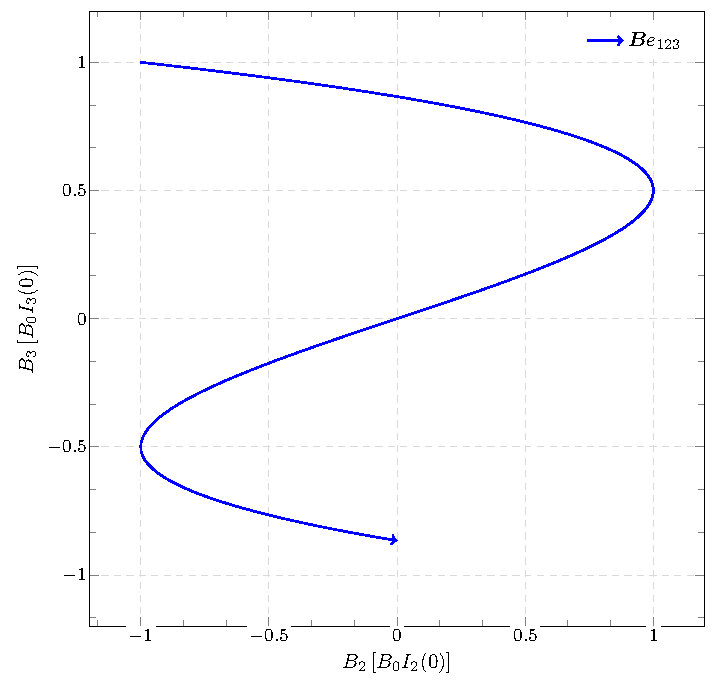
\includegraphics[width=\linewidth]{../Figures/Uniform-Field/B-sin-sin.pdf}
		\caption{Señales sinusoidales.}
		\label{fig:b_sin_sin}
	\end{subfigure}
	\hfill
	\begin{subfigure}{0.32\linewidth}
		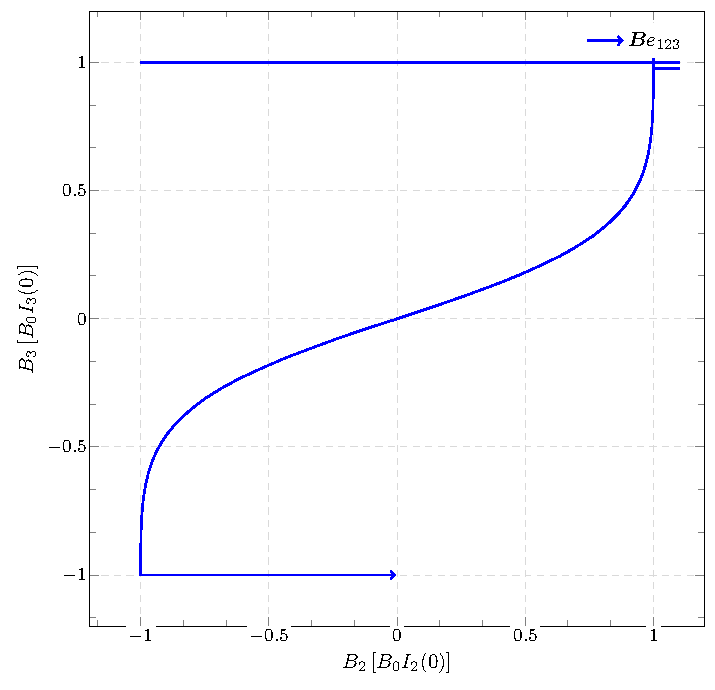
\includegraphics[width=\linewidth]{../Figures/Uniform-Field/B-square-square.pdf}
		\caption{Señales cuadradas.}
		\label{fig:b_sqr_sqr}
	\end{subfigure}
	\hfill
	\begin{subfigure}{0.32\linewidth}
		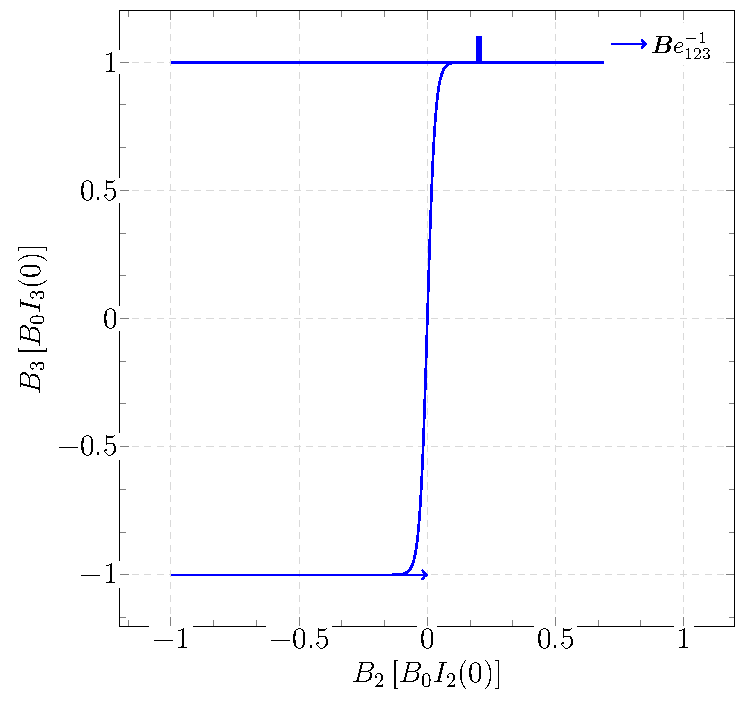
\includegraphics[width=\linewidth]{../Figures/Uniform-Field/B-sin-square.pdf}
		\caption{Señal sinusoidal y cuadrada.}
		\label{fig:b_sin_sqr}
	\end{subfigure}
	\caption{Evolución del vector de campo magnético $\boldsymbol{B}^*$ en
		el plano $yz$ para distintas formas de onda de la corriente. Se
	muestra una razón de frecuencias de 3:1 y un desfase $\phi=0$.}
	\label{fig:B_fields}
\end{figure}

\subsubsection{Análisis del Campo Eléctrico Inducido}
\label{sssec:dinamica_e}

El campo eléctrico inducido $\boldsymbol{E}$ depende de la tasa de cambio
del campo magnético, $\partial_t \boldsymbol{B}$. Su magnitud es, por
ende, proporcional a la frecuencia de las corrientes de alimentación.
A continuación, se cuantifica su efecto en comparación con el campo
magnético para las condiciones específicas del experimento.

La razón entre las magnitudes de las fuerzas eléctrica y magnética es:
%
$$
\frac{|\boldsymbol{F}_E|}{|\boldsymbol{F}_B|} \approx
\frac{|\boldsymbol{E}|}{v |\boldsymbol{B}|}
$$
%
Para una señal sinusoidal, $|\boldsymbol{E}| \approx R \omega |\boldsymbol{B}|$,
donde $R$ es el radio de las bobinas, $\omega$ la frecuencia angular y $v$
la velocidad del electrón. La razón de fuerzas es entonces $\approx R\omega/v$.

Con los parámetros del montaje, se tiene:
%
\begin{itemize}
	\item Una frecuencia $f \approx \qty{50}{\hertz}$, que implica una frecuencia
		angular $\omega = 2\pi f \approx \qty{314}{\radian\per\second}$.
	\item Una energía cinética de $\qty{4.1}{\kilo\eV}$, que corresponde a una
		velocidad del electrón de $v \approx 0.1c$.
	\item Un radio de bobinas $R$ del orden de $\qty{6.2}{\centi\meter}$.
\end{itemize}
%
Sustituyendo estos valores se obtiene:
%
$$
\frac{|\boldsymbol{F}_E|}{|\boldsymbol{F}_B|} \approx \frac{R\omega}{v}
\approx 10^{-7}
$$
%
Este resultado numérico, de orden $10^{-7}$, confirma de manera
contundente que la fuerza magnética es aproximadamente \emph{diez millones} de
veces mayor que la fuerza eléctrica. Por lo tanto, es una aproximación
justificada considerar que la dinámica es gobernada
exclusivamente por el campo magnético, omitiendo el término de
$\boldsymbol{E}$ en el modelo.


\subsection{Modelo II: Campo a partir de la Ley de Biot-Savart}
\label{ssec:modelo_biot_savart}

En este modelo, se abandona la aproximación de campo uniforme para calcular
el campo magnético de forma más fundamental. Se utiliza la ley de
Biot-Savart para cada espira de las bobinas.

Se considera una única espira circular de radio $R$ en el plano inferior
del par de bobinas del eje $z$, ubicado en $z = -R/2$. Su geometría se
parametriza por el vector $\boldsymbol{l}_1(\theta)$:
%
\begin{equation}
	\boldsymbol{l}_1(\theta) = R \cos(\theta) e_1 + R \sin(\theta) e_2
	- \frac{R}{2} e_3.
\end{equation}
%
El campo magnético bivectorial que esta espira genera en un punto
arbitrario $\boldsymbol{r} = x_1 e_1 + x_2 e_2 + x_3 e_3$ está dado por la
ley de Biot-Savart, integrada sobre el lazo cerrado:
%
\begin{equation}
	\boldsymbol{B}_1(t, \boldsymbol{r}) = \frac{\mu_0 N I_1(t)}{4 \pi} \oint
	\frac{\mathrm{d}\boldsymbol{l}_1 \wedge (\boldsymbol{r} - \boldsymbol{l}_1)}
	{|\boldsymbol{r} - \boldsymbol{l}_1|^3},
	\label{eq:biot_savart_bivector}
\end{equation}
%
donde $N$ es el número de vueltas de la bobina y $I_1(t)$ es la corriente
que circula por ella.

El campo de la segunda bobina del par, ubicada coaxialmente en $z = +R/2$,
se deduce por simetría. Si la corriente $I_2(t)$ en la bobina superior
circula en la misma dirección que $I_1(t)$ (configuración Helmholtz),
la relación de simetría es distinta; no obstante, la forma del campo
resultante es bien conocida por su alta uniformidad en la región
central, para la cual existen soluciones analíticas estándar.

Por otro lado, si se considera una configuración anti-Helmholtz (corrientes
opuestas), el sistema presenta una simetría de inversión. En este caso, el
campo de la segunda bobina, $\boldsymbol{B}_2$, se relaciona con el de la
primera mediante una reflexión sobre el origen:
%
\begin{equation}
	\boldsymbol{B}_2(t, \boldsymbol{r}) =
	-\boldsymbol{B}_1(t, -\boldsymbol{r}, I_1(t)).
	\label{eq:simetria_inversion_B}
\end{equation}
%
Esta importante simplificación surge de la simetría axial de las bobinas
combinada con la simetría de paridad de la configuración. El campo total
del par de bobinas es entonces la superposición
$\boldsymbol{B}_{\text{par}}(t, \boldsymbol{r}) = \boldsymbol{B}_1 + \boldsymbol{B}_2$.
El mismo análisis se aplica a los otros pares de bobinas a lo largo de los
demás ejes.

\subsubsection{Campo Eléctrico en la Configuración anti-Helmholtz}
\label{sssec:campo_electrico_ah}

Aunque el análisis cuantitativo previo ya justifica la dominancia de la
fuerza magnética, la configuración anti-Helmholtz presenta una propiedad
de simetría que refuerza esta conclusión.

Debido a la simetría axial y de inversión de esta configuración, el
potencial vectorial magnético $\boldsymbol{A}$ es nulo a lo largo del eje
de las bobinas. Como consecuencia directa, el campo eléctrico inducido,
$\boldsymbol{E} = -\partial_t \boldsymbol{A}$, también es cero sobre dicho
eje. Esto implica que en la región central del montaje, la más relevante
para la trayectoria del haz, el efecto del campo eléctrico es aún más
despreciable.

\subsection{Modelo III: Aproximación de Campo Cuadrupolar}
\label{ssec:modelo_cuadrupolar}

El campo generado por un par de bobinas en configuración anti-Helmholtz
puede ser aproximado cerca de su centro por un campo de gradiente lineal,
característico de un cuadrupolo magnético. Al superponer los campos de
varios pares, se obtiene un campo cuadrupolar tridimensional.

Una aproximación lineal para dicho campo es:
%
\begin{equation}
	\boldsymbol{B}(\boldsymbol{r}, t) = b(t)
	\left( - x_1 e_{23} + \frac{1}{2} x_2 e_{31} + \frac{1}{2} x_3 e_{12} \right).
	\label{eq:quadrupole_field}
\end{equation}
%
Este campo satisface la condición de Maxwell $\langle \nabla \boldsymbol{B} \rangle_3 = 0$.
La dependencia temporal del campo se engloba en el coeficiente $b(t)$.

Este tipo de campo de gradiente es la base de las trampas magnéticas.
Cuando las corrientes son tales que el campo apunta hacia el origen, se
crea un pozo de potencial que confina el haz (efecto de \emph{enfoque}).
Inversamente, si el campo apunta hacia afuera, las partículas son
repelidas del centro (\emph{desenfoque}).

Con corrientes alternas, el sistema oscila entre un estado de enfoque y
desenfoque. Esto puede resultar en un confinamiento dinámico neto del
haz, un principio análogo al de las trampas de Paul para partículas
cargadas.

